\subsection{Documentazione}

\subsubsection{Scopo}
Lo scopo di questo processo è quello di redigere e mantenere la documentazione durante tutto il ciclo di vita del software.
I documenti formali che verranno presentati saranno suddivisi in due categorie:

\begin{itemize}
\item[•] \textbf{Interni}:
	\begin{list}{$\circ$}{}
		\item \textbf{Norme di progetto}: lo scopo del documento è di stabilire convenzioni e norme che il team SWEight deve seguire durante tutto il progetto;	
	    \item \textbf{Studio di fattibilità}: il documento presenta il processo che ha portato il team alla scelta del capitolato, riportando le motivazioni di preferenza o rifiuto di ogni capitolato;
    \end{list} 
\item[•] \textbf{Esterni}:
	\begin{list}{$\circ$}{}
		\item \textbf{Piano di progetto}: documento per l’analisi e la pianificazione della gestione delle risorse di tempo e umane;
		\item \textbf{Piano di qualifica}: documento che descrive standard e obiettivi che il gruppo deve raggiungere per garantire la qualità di processo e prodotto;
		\item \textbf{Glossario}: documento che raccoglie i termini appartenenti ad un ambito specifico e circoscritto. Contiene la spiegazione dei termini desueti o specialistici utilizzati nei documenti;
		\item \textbf{Analisi dei requisiti}: documento che contiene l’analisi dei casi d’uso del prodotto e i diagrammi di interazioni previste con l'utente;
		\item \textbf{Manuale Utente}: documento che fornisce all'utente finale istruzioni su come usare il prodotto software;
		\item \textbf{Manuale Sviluppatore}: documento che fornisce allo sviluppatore indicazioni utili per comprendere ed espandere il prodotto software. 
	\end{list}
\end{itemize}
\subsubsection{Classificazione dei documenti} \label{documenti}


\paragraph{Documenti informali}\mbox{}\\
Tutti i documenti non ancora approvati dal \textit{Responsabile di progetto} sono da ritenersi informali quindi ad uso esclusivamente interno.

\paragraph{Documenti formali}\mbox{}\\
Un documento diventa formale in seguito all'approvazione da parte del \textit{Responsabile di progetto}. Solo i documenti formali possono essere divulgati all'esterno del gruppo. Prima di poter essere approvato un documento deve essere verificato. 

\paragraph{Verbali}\mbox{}\\ 
\label{sec:verbali}
Per ogni incontro deve essere nominato un segretario che si occuperà della stesura di un verbale. Il verbale deve contenere i seguenti punti: 
\begin{itemize}
\item \textbf{Estremi della riunione}: 
	\begin{list}{$\circ$}{}
		\item Motivazione;
		\item Luogo;		
		\item Data;
		\item Partecipanti del gruppo;
		\item Ora; 
		\item Segretario.
	\end{list}
\item \textbf{Ordine del giorno}: lista degli argomenti che saranno oggetto di discussione; 
\item \textbf{Resoconto}: verbale effettivo degli argomenti discussi. Il tracciamento delle decisioni prese sarà fatto nel seguente modo: ogni decisione sarà identificata da un codice: \textit{VER-NumeroVerbale-Data.x} dove \textit{NumeroVerbale} è il numero assegnato al verbale, \textit{Data} è la data in cui è stato svolto l'incontro e \textit{x} è un numero sequenziale.
\end{itemize}
Una volta approvato dal \textit{Responsabile di progetto}, il verbale deve essere distribuito a tutti i componenti del gruppo. In caso di verbale esterno il verbale dovrà essere inviato anche al proponente. 
I nomi dei file dei verbali devono rispettare il seguente formato:
\begin{center}
Verbale-[numeroVerbale]-[T]-[Data].pdf
\end{center}
dove: 
\begin{itemize}
\item \textbf{numeroVerbale}: è l'identificativo numerico del verbale;
\item \textbf{T} è la tipologia del verbale che si divide in:
\begin{list}{$\circ$}{}
\item \textbf{I}: interni;
\item \textbf{E}: esterni.
\end{list}
\item \textbf{Data}: è la data in cui è stato svolto il verbale nel formato descritto nel paragrafo \hyperref[sec:Formati]{§4.1.6.1}.
\end{itemize}

\subsubsection{Nome dei documenti}\mbox{}\\
I nomi dei documenti devono:
\begin{itemize}
\item Iniziare con la lettera maiuscola;
\item Se composti da più parole anche esse devono avere la lettera maiuscola;
\item Dopo il nome testuale, segue un carattere di underscore;
\item Infine si indica la versione come descritto in \hyperref[sec:documentversion]{§4.1.4}.
\end{itemize}
Esempio:
\begin{center}
\texttt{NomeDocumento\_v1.0.0}
\end{center}
I documenti devono essere esportati in formato PDF.

\subsubsection{Template}
Per semplificare e standardizzare la stesura dei documenti previsti è stato creato un template \LaTeX{} contenente tutte le impostazioni per la struttura grafica e lo stile di formattazione. Ogni membro del team deve obbligatoriamente utilizzare questo {template}\ped{G}.
Quest'ultimo è disponibile all'interno dell'omonima cartella ed è denominato "SWEightStyle.sty", e dev'essere importato all'interno del documento \LaTeX{} tramite la direttiva di inclusione di un pacchetto.
\subsubsection{Versioni}
\label{sec:documentversion}
Per ogni documento deve essere specificata obbligatoriamente la versione nella seguente forma: 
\begin{center}
\textbf{X.Y.Z}
\end{center}
Dove X, Y, e Z sono interi non negativi. X viene incrementata ad ogni revisione, Y viene incrementata ogni qualvolta venga inserito un nuovo capitolo, infine Z determina le modifiche al documento. Ogni elemento deve incrementare indipendentemente. Per esempio: 1.9.0 $\rightarrow$ 1.10.0 $\rightarrow$ 1.11.0 .

%\begin{itemize}
%\item[•]La versione Major zero (0.y.z) è per lo sviluppo iniziale;
%\item[•]X: la versione Major (X.y.z | X > 0) identifica la versione di rilascio. Deve essere incrementata se è stata introdotta qualsiasi modifica non retrocompatibile. Le versioni Patch e Minor devono essere reimpostate a 0 quando la versione Major è incrementata;
%\item[•]Y: la versione Minor (x.Y.z | x > 0) deve essere incrementata se è stata introdotta una nuova funzionalità. La versione Patch deve essere reimpostata a 0 quando la versione Minor è incrementata;
%\item[•] Z: la versione Patch (x.y.Z | x > 0) deve essere incrementata solo se sono state introdotte correzioni retrocompatibili di bug. Una correzione di un bug è definita come una modifica interna che corregge un comportamento errato.
%\end{itemize}
%Una volta che un pacchetto versionato è stato rilasciato, i contenuti di quella versione non devono essere modificati. Qualsiasi modifica deve essere rilasciata come una nuova versione.

\subsubsection{Struttura}
Ogni documento deve essere realizzato a partire dal template descritto precedentemente, la cui struttura non deve essere modificata, ad eccezione dei verbali e della lettera di presentazione, dovrà essere composta da:
\begin{itemize}
\item[•] \textbf{Frontespizio}: questa sezione si trova nella prima pagina di ogni documento e deve contenere:
     \begin{list}{$\circ$}{}
		\item \textbf{Logo}: il logo del gruppo;
		\item \textbf{Titolo}: il titolo del documento;
		\item \textbf{Nome del gruppo};
		\item \textbf{Nome del progetto};
		\item \textbf{E-mail}: indirizzo di posta elettronica in comune per le comunicazioni interne ed esterne;
		\item \textbf{Versione}: versione del documento;
		\item \textbf{Approvatore}: \textit{Responsabile di progetto};
		\item \textbf{Redattori}: \textit{Redattori} del documento;
		\item \textbf{Verificatori}: \textit{Verificatori} del documento;
		\item \textbf{Uso}: interno o esterno;
		\item \textbf{Distribuzione}: destinatari del documento;
		\item \textbf{Descrizione}: breve descrizione del documento;		
	\end{list}
\item[•] \textbf{Registro delle modifiche}: il registro delle modifiche deve essere riportato subito dopo il frontespizio. Esso deve contenere, in forma tabellare: versione del documento, data di salvataggio, descrizione della nuova versione, nominativo e ruolo;
\item[•] \textbf{Indice}: contiene il nome di tutti i capitoli, sezioni e sottosezioni seguiti dal numero della pagina iniziale;
\item[•] \textbf{Indice delle immagini}: nel caso in cui il documento contenga immagini;
\item[•] \textbf{Indice delle tabelle}: nel caso in cui il documento contenga tabelle;
\item[•] \textbf{Introduzione}: contiene lo scopo del documento, una breve descrizione ed i vari riferimenti normativi e informativi utili al lettore;
\item[•] \textbf{Contenuto del documento}.
\end{itemize}



\paragraph{Formattazione delle pagine}\mbox{}\\
Ogni pagina, escluso il frontespizio ed indice, devono contenere:
\begin{itemize}
	\item[•] \textbf{Intestazione}:
	\begin{list}{$\circ$}{}
		\item Logo del gruppo (a sinistra);
		\item Numero del capitolo corrente seguito dal nome (a destra).
	\end{list}
	\item[•] \textbf{Piè di pagina}:
	\begin{list}{$\circ$}{}
	\item Nome e versione del documento (sinistra);
	\item Numero pagina, in formato “N di M” dove N è la pagina corrente ed M è il numero di pagine totali.
	\end{list} 
\end{itemize}

\subsubsection{Norme Tipografiche}
\begin{itemize}
\item[•] \textbf{Maiuscolo}: l'uso del maiuscolo è obbligatorio nei seguenti casi:
	\begin{list}{$\circ$}{}
	\item All'inizio di ogni elemento di un elenco puntato;
	\item Nella scrittura degli acronimi;
	\item Dopo il punto, punto di domanda, punto esclamativo;
	\item Per i ruoli di progetto, i nomi dei documenti, le fasi di progetto, revisioni di progetto oltre a dove previsto dalla lingua italiana;
	\end{list}
\item[•] \textbf{Grassetto}: il grassetto può essere utilizzato solo per evidenziare l’oggetto trattato di un elenco puntato e per le parole chiave;
\item[•] \textbf{Collegamenti}: tutti i collegamenti, URL, devono essere di colore rosso;
\item[•] \textbf{Riferimenti a sezioni}: i riferimenti interni al documento devono riportare il numero della sezione, preceduto dal simbolo di paragrafo (esempio  §2.1.3);
\item[•] \textbf{Corsivo}: il corsivo deve essere utilizzato nei seguenti casi:
\begin{list}{$\circ$}{}
	\item \textbf{Ruoli}: in ogni nome di ruolo;
	\item \textbf{Documenti}: in ogni nome di documento;
	\item \textbf{Citazioni}: in ogni citazione.
\end{list}

\item[•] \textbf{Codice}: i frammenti di codice devono essere racchiusi in un riquadro di colore nero;
\item[•] \textbf{Glossario}: per contrassegnare una parola che è presente nel glossario è necessario aggiungere una G maiuscola al pedice della parola (ad esempio: {termine}\ped{G});
\item[•] \textbf{Elenchi puntati}:
\begin{itemize}
	\item Ogni elemento dell'elenco deve terminare con il punto e virgola, ad eccezione dell'ultimo elemento che deve terminare con il punto;
	\item \textbf{Elenco puntato non ordinato}:
	Gli elementi di primo livello devono avere come stile un pallino pieno nero, quelli di secondo livello un pallino nero vuoto. Elementi di livello successivo al secondo devono alternare lo stile del primo e del secondo livello.
	\item \textbf{Elenco puntato ordinato}:
	Gli elementi di primo livello devono avere come stile un numero progressivo, mentre quelli di secondo livello una lettera racchiusa all'interno di parentesi graffe;
	\end{itemize}
	\item[•] \textbf{Citazioni}: ogni citazione deve essere accompagnata dal riferimento bibliografico.
\end{itemize}

\paragraph{Formati}\mbox{}\\ \label{sec:Formati}
\begin{itemize}
	\item \textbf{Date}: ogni data deve rispettare lo standard internazionale ISO 8601:2004, che prevede la seguente convenzione:
	\begin{center}
	AAAA-MM-GG
	\end{center}
	dove: 
	\begin{itemize}
		\item[$\circ$] \textbf{AAAA}: rappresenta il formato dell'anno scritto con quattro cifre;
		\item[$\circ$] \textbf{MM}: rappresenta il formato del mese scritto con due cifre;
		\item[$\circ$] \textbf{GG}: rappresenta il formato del giorno scritto con due cifre;
		\end{itemize}
		\item \textbf{Orari}: se presenti, gli orari fanno riferimento anch'essi allo standard internazionale ISO 8601:2004:
		\begin{center}
		HH:MM
		\end{center}
		dove:
		\begin{itemize}
		\item[$\circ$] \textbf{HH}: rappresenta l'ora espressa con due cifre il cui valore è compreso tra 00 e 23;
		\item[$\circ$] \textbf{MM}: rappresenta i minuti espressi con due cifre il cui valore è compresi tra 00 e 59.
	\end{itemize}
\end{itemize}

\subsubsection{Componenti grafiche}

\paragraph{Tabelle}\mbox{}\\
Tutte le tabelle devono avere un indice univoco che la identifichi all’interno del documento ed una breve descrizione posizionata sotto di essa. Le intestazioni delle tabelle devono essere in grassetto.
Le righe possono avere colori alternati per facilitarne la lettura.
\paragraph{Immagini}\mbox{}\\
Tutte le immagini inserite nei vari documenti devono avere un eguale e sufficiente margine orizzontale e verticale in modo da non ridurre la leggibilità del testo. Ogni immagine deve anch'essa avere un indice univoco che la contraddistingua nell'intero documento.
In particolare le immagini dovranno rispettare le seguenti proprietà, salvo indicato diversamente:
\begin{itemize}
\item[•] \textbf{Nome}: deve rispettare la {notazione a cammello}\ped{G};
\item[•] \textbf{Formato}: è preferibile utilizzare il formato PNG, ma è accettato anche il PDF in quanto scalabile;
\item[•] \textbf{Importazione in \LaTeX}: quando importata nel documento, l'immagine dev'essere collocata all'interno del tag figure, accompagnata da una descrizione e con lunghezza massima uguale a 17cm;
\item[•] \textbf{Posizionamento}: preferibilmente deve essere centrata orizzontalmente.
\end{itemize}

\subparagraph{Esportare immagini in Astah}\mbox{}\\
Per esportare i diagrammi in Astah, dopo aver completato il diagramma, selezionare: 
\begin{center}
	$Tools \rightarrow Export\ image \rightarrow Current\ Diagram \rightarrow PNG$.
\end{center}

L'immagine rappresentante l'UML deve avere le seguenti caratteristiche:
\begin{itemize}
\item \textbf{Nome file}: UC\texttt{Codice Identificativo}, privo di "."\\
Ad esempio: UC4.2.png $\rightarrow$ UC42.png;
\item \textbf{Formato file immagine}: \texttt{.png};
\item \textbf{Massima larghezza}: 17cm;
\item \textbf{Didascalia:} figura con codice caso d'uso;
\item \textbf{Salvataggio:} Il file deve essere salvato all'interno del folder img, destinato alle immagini.
\end{itemize}
Inoltre, anche il file con estensione asta deve essere salvato nella cartella predisposta al fine di permetterne modifiche successivamente. 
Per la realizzazione dell'Analisi dei Requisiti la cartella destinata al salvataggio dei diagrammi modificabili è: "Casi d'uso", reperibile all'interno del {branch}\ped{G} Analisi dei Requisiti. Il nome del diagramma deve essere il medesimo dell'immagine esportata.

\subsubsection{Strumenti di supporto} 

\paragraph{\LaTeX{}}\mbox{}\\
L'intera documentazione deve essere prodotta utilizzando il {linguaggio di markup}\ped{G} \LaTeX{}, scelto dal team per i seguenti motivi:
\begin{itemize}
\item[•] Gestisce elegantemente e con facilità gli indici, i pedici, i riferimenti ed il glossario;
\item[•] È un linguaggio che supporta il {versionamento}\ped{G};
\item[•] Permette la suddivisione del documento in parti che rappresentano le varie sezioni facilitando la stesura.
\end{itemize}
Per utilizzare \LaTeX{} è necessario installare il compilatore pdflatex, integrato in un software come TexLive reperibile all'indirizzo  \url{https://www.tug.org/texlive/}. Quest'ultimo è {cross platform}\ped{G}, {open source}\ped{G} e gratuito. Si consiglia l'installazione del pacchetto completo per evitare di installare pacchetti successivamente.
Per la stesura del documento si consiglia Texmaker, il quale presenta le seguenti peculiarità:
\begin{itemize}
	\item[•] Compilatore e visualizzatore {PDF}\ped{G} per il documento prodotto;
	\item[•] Evidenziamento della sintassi;
	\item[•] Completamento automatico.
\end{itemize}  
Il software è reperibile all'indirizzo \url{http://www.xm1math.net/texmaker/}, è cross-platform ed è gratuito.

\paragraph{GNU Aspell}\mbox{}\\
Al termine della stesura dei documenti, prima della fase di verifica del documento, un \textit{Redattore} deve effettuare un controllo ortografico sui file tex tramite GNU Aspell, reperibile al seguente link:
\begin{center}
	\url{http://aspell.net/}
\end{center}
Il dizionario italiano per l'applicativo, insieme alle istruzioni per l'installazione, è disponibile al seguente link:
\begin{center}
	\url{https://ftp.gnu.org/gnu/aspell/dict/0index.html}
\end{center}
Il programma esegue da terminale con il seguente comando:
\begin{center}
	\texttt{aspell -c -t nomeFile.tex -d it}
\end{center}

\paragraph{MAGIC}\mbox{}\\
Per il calcolo dell'indice di Gulpease, il gruppo \gruppo \space si avvale dello script MAGIC (Magic Automatic Gulpease Index Calulator) sviluppato internamente.
Il tool esegue automaticamente ogni giorno e svolge i seguenti step:
\begin{enumerate}
	\item Compilazione di tutti i documenti;
	\item Calcolo dell'indice di Gulpease per ogni documento;
	\item Salvataggio dei valori ottenuti in foglio di calcolo Google.
\end{enumerate}
I valori inseriti sono automaticamente plottati in un grafico, che permette ai verificatori di monitorare celermente il livello di leggibilità di ogni documento.

\subsubsection{Ciclo di vita dei documenti}
Per gestire il ciclo di vita dei documenti, deve essere utilizzato il servizio di task offerto da Asana, come descritto nella sezione \hyperref[sec:documentversion]{§5.2} gestione dell'infrastruttura.
\begin{enumerate}
\item Il \textit{Responsabile di progetto} crea il task, assegna i \textit{Redattori} ed i \textit{Verificatori}, e lo mette nella colonna "To Do" ;
\item Quando i \textit{Redattori} assegnati iniziano la stesura del documento spostano il task nella colonna "In progress";
\item Finita l'attività di scrittura il task deve essere spostato in "Need Review"
\item I \textit{Verificatori} assegnati controllano il documento decidendo se:
	\begin{enumerate}
	 	\item Accettarlo, e muoverlo in "Done";
	 	\item Non accettarlo e rimetterlo in "In Progress", lasciando un commento al task;
	\end{enumerate}
\item Se non accettato, i \textit{Redattori} devono apportare le modifiche descritte dai \textit{Verificatori};
\item Se accettato, il documento giunge al \textit{Responsabile di progetto} che può:
\begin{enumerate}
	\item Approvarlo, rendendo il documento formale e marcarlo come completato.
	\item Non approvarlo, fornendo le opportune motivazioni come commento al task e spostandolo in "To Do";
\end{enumerate}
\item Se approvato, sarà compito dell'\textit{Amministratore di Progetto} effettuare il merge.
\end{enumerate}
\begin{figure}[H]
\centering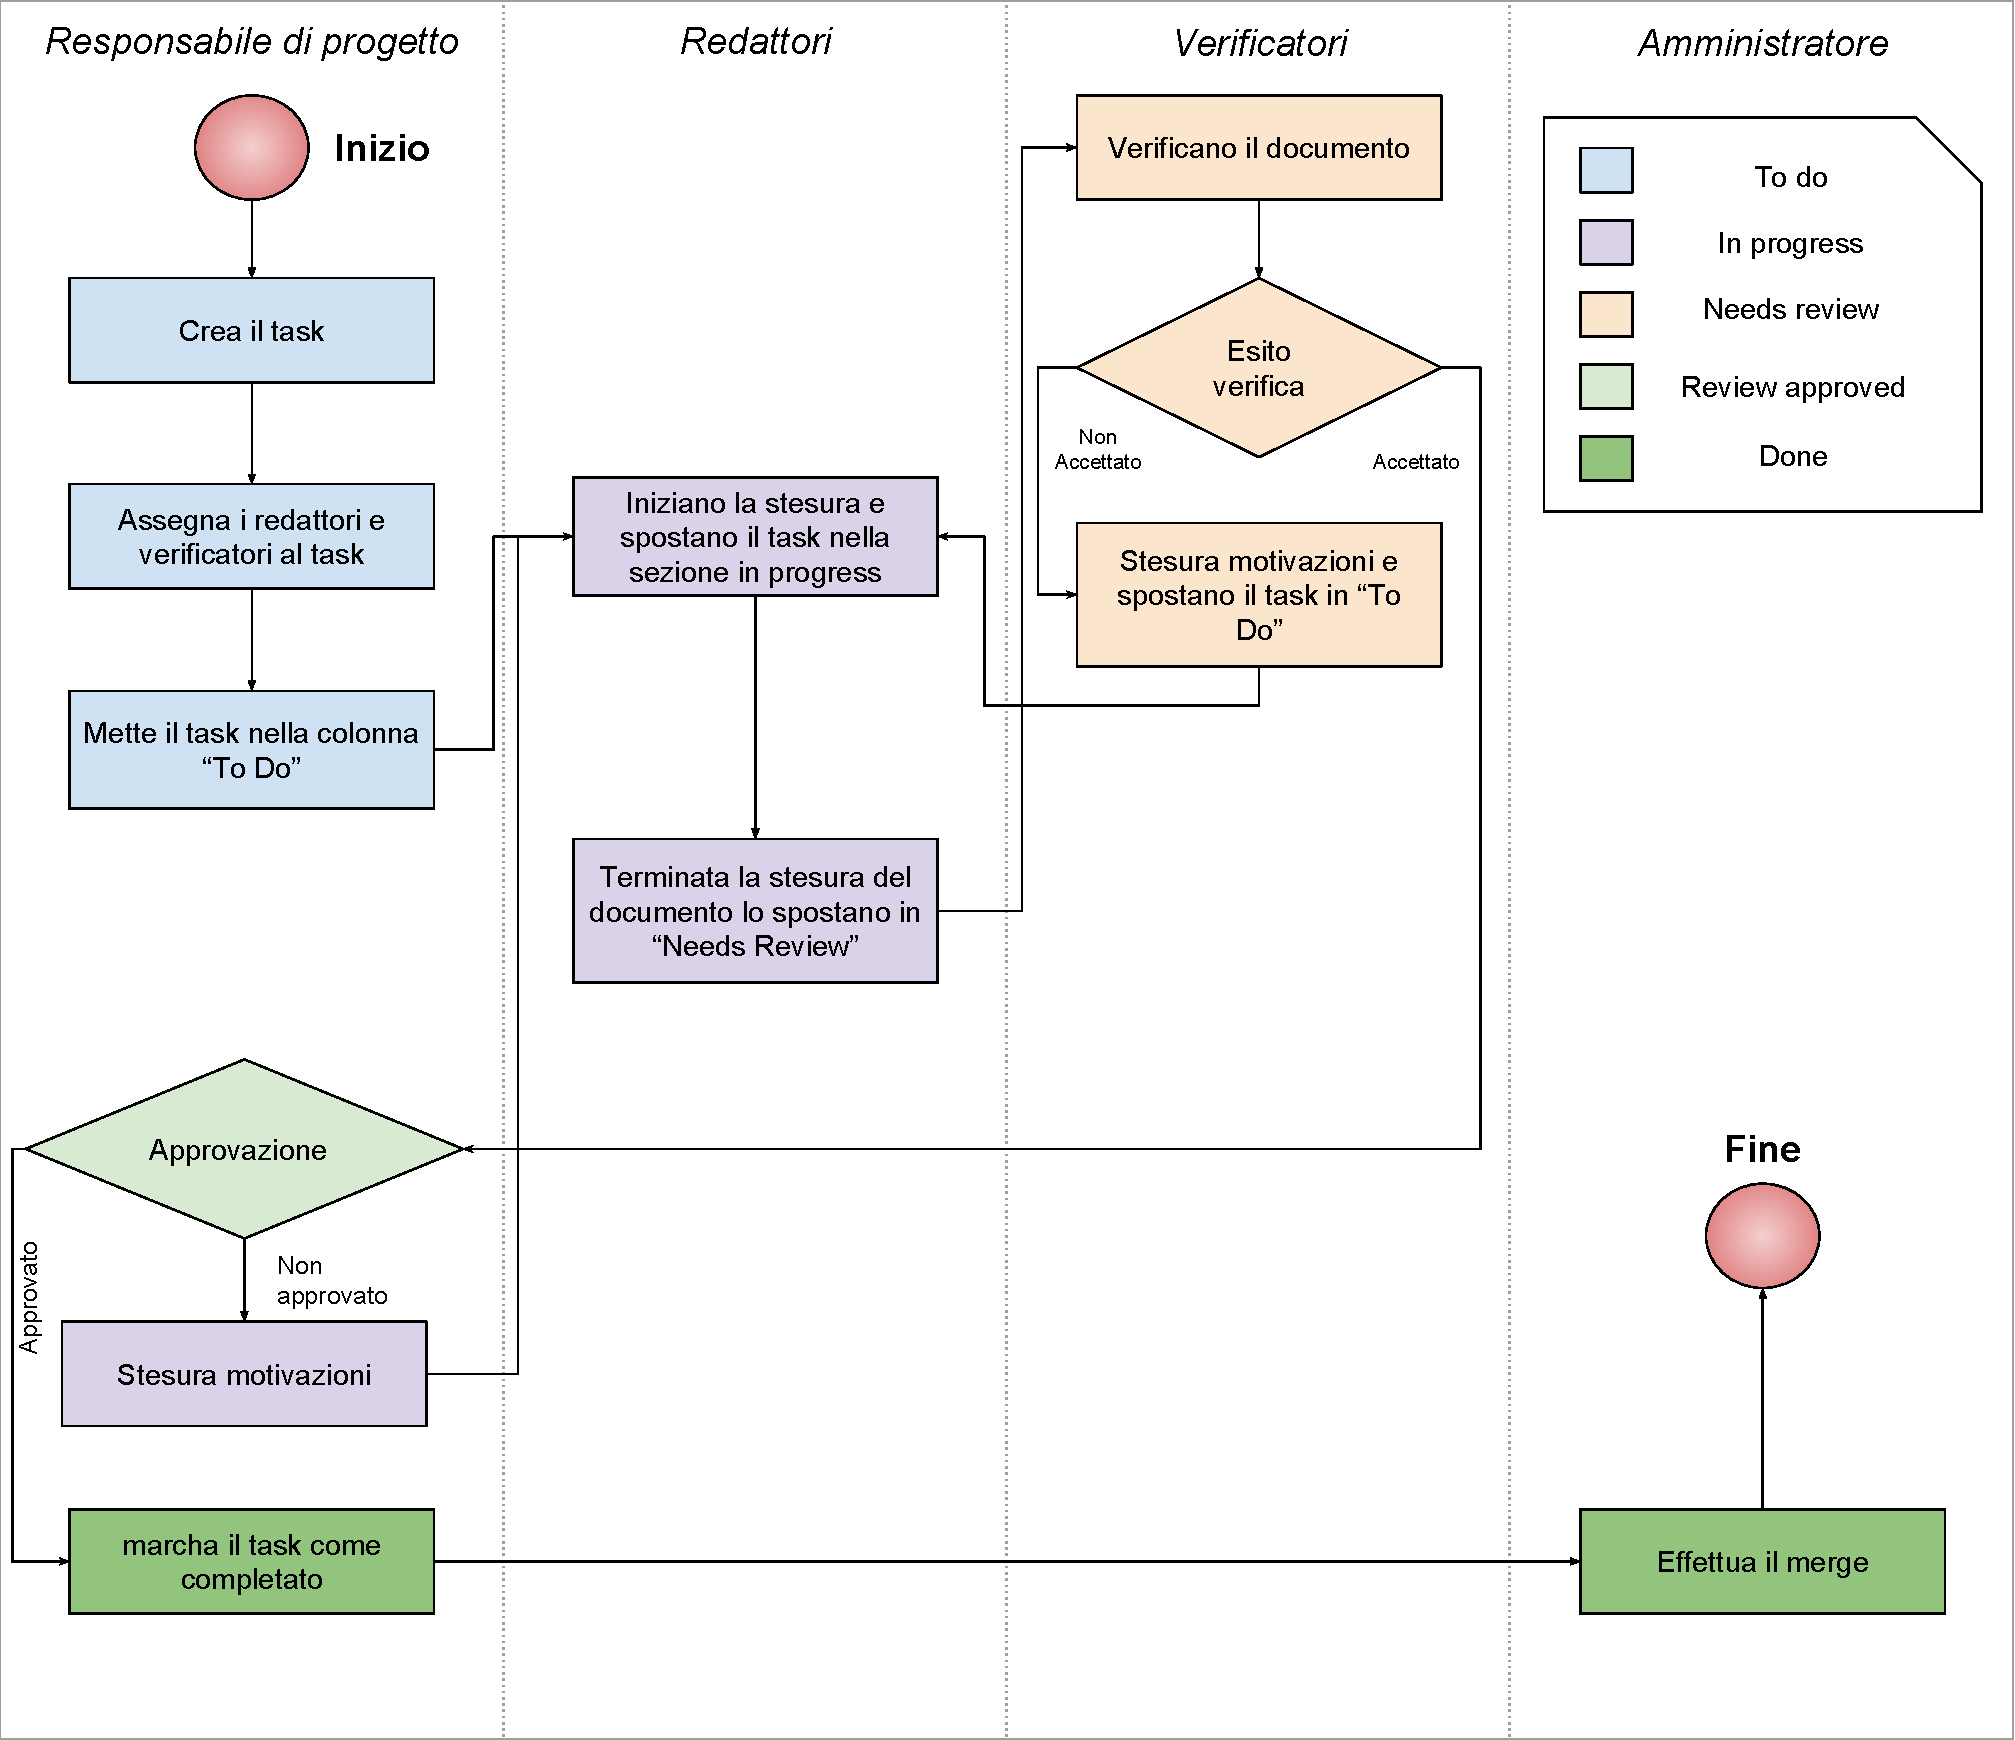
\includegraphics[width=17cm,trim=2 2 2 2, clip]{img/cicloVitaDocumentoAsana.pdf}
\caption{Ciclo di vita di un documento}
\label{fig:document_lifecycle}
\end{figure}

\paragraph{Diagrammi UML}\mbox{}\\
Il software che deve essere utilizzato per la creazione dei diagrammi UML è Astah versione 8.0.0, gli \textit{Analisti} devono utilizzare la documentazione del software per il suo studio e utilizzo.
Ogni diagramma di caso d’uso è identificato in alto a sinistra dal suo codice identificativo e dal nome.

\subsection{Qualità}
\subsubsection{Scopo}
Questa sezione descrive le classificazioni e le formule per il calcolo delle metriche necessarie per assicurare la qualità.

\subsubsection{Classificazione delle metriche}
Per garantire la qualità del lavoro gli Amministratori hanno definito delle metriche, che devono però rispettare la seguente notazione M[categoria][numero] dove:
\begin{itemize}
	\item{categoria}: indica la categoria della metrica, può assume i valori:
	\begin{itemize}
		\item D per indicare le metriche di documenti;
		\item S per indicare le metriche di software;
		\item P per indicare le metriche di processi.
	\end{itemize}
	\item{numero}: identifica in maniera univoca la metrica in ogni categoria, assume un valore intero a 3 tre cifre incrementale a partire da 1.
\end{itemize}
Ad esempio la prima metrica sui documenti sarà classificata in questo modo:
\begin{center}
	MD001
\end{center}

\paragraph{Metriche Documenti}\mbox{}\\
Le metriche presentate in questa sezione hanno come scopo fornire delle metriche per garantire un buon livello di leggibilità dei documenti.


\subparagraph{MD001 - Indice Gulpease}\mbox{}\\
L'Indice Gulpease è un indice di leggibilità di un testo tarato sulla lingua italiana. Rispetto ad altri ha il vantaggio di utilizzare la lunghezza delle parole in lettere anziché in sillabe, semplificandone il calcolo automatico.
L'indice di Gulpease considera due variabili linguistiche: la lunghezza della parola e la lunghezza della frase rispetto al numero delle lettere.
L'indice di Gulpease può assumere valori fra 0 e 100 e si calcola come segue:
\[
IG = 89 + \frac{300 \cdot \textit{(numero delle frasi)} - 10 \cdot \textit{(numero delle lettere)}}{\textit{numero delle parole}}
\]

\paragraph{Metriche Software}\mbox{}\\
Le metriche presentate in questa sezione hanno come scopo fornire delle metriche per garantire un buon livello di qualità del software.
\subparagraph{MS001 - Numero di Metodi}\mbox{}\\
Numero medio di metodi contenuti nelle classi di un package. Un numero di metodi troppo alto può indicare la necessità di scomporre una classe. Un numero di metodi troppo basso, d'altro canto, deve far riflettere sull'effettiva utilità della classe presa in esame.
\subparagraph{MS002 - Numero di Parametri}\mbox{}\\
Numero di parametri passati a un metodo. Un eccessivo numero di parametri passati ad un metodo può indicare un'eccessiva complessità dello stesso, che va scomposto o quanto meno ripensato.
\subparagraph{MS003 - Funzioni di interfaccia per package}\mbox{}\\
Numero di funzioni che un package espone. Un valore troppo elevato potrebbe indicare un errore di progettazione.
\subparagraph{MS004 - Complessità Ciclomatica}\mbox{}\\
La Complessità Ciclomatica (CC) è una metrica software che misura la complessità di un programma contando il numero di cammini linearmente indipendenti attraverso il grafo di controllo di flusso. In questo grafo, i nodi corrispondono a gruppi indivisibili di istruzioni, mentre gli archi connettono due nodi se il secondo gruppo di istruzioni può essere eseguito immediatamente dopo il primo gruppo: sono quindi responsabili dell'aumento della CC i punti decisionali, \emph{if} e \emph{for}.
Tenere bassa la CC può portare a vari vantaggi:
\begin{itemize}
	\item Minore complessità durante lo sviluppo;
	\item Maggior facilità nell'aumentare la code coverage in fase di test;
	\item Maggior coesione del codice.
\end{itemize}
La Complessità Ciclomatica è calcolata come segue:
\[
CC = v(G) = e - n + 2p
\]
dove:
\begin{itemize}
	\item \emph{e} = numero di archi del grafo;
	\item \emph{n} = numero di nodi del grafo;
	\item \emph{p} = numero di componenti connesse.
\end{itemize}
\subparagraph{MS005 - Campi dati per classe}\mbox{}\\
Numero di campi dati contenuti da una classe. Una classe con troppi campi dati può essere sintomo di cattiva progettazione e va ripensata.
\subparagraph{MS006 - Commenti per linee di codice}\mbox{}\\
Rapporto fra numero di righe di commento e numero totale di righe (vuote escluse). Un codice ben commentato può essere compreso più facilmente e velocemente, facilitando le operazioni di manutenzione.
\subparagraph{MS007 - Code Coverage}\mbox{}\\
Percentuale delle linee di codice coperte dai test. Avere codice coperto da test riduce la possibilità di introdurre errori nel prodotto.
\subparagraph{MS008 - Superamento test}\mbox{}\\
Percentuale di test superati. Per avere un prodotto di qualità, è necessario che esso superi i test prestabiliti.
\subparagraph{MS009 - Requisiti obbligatori soddisfatti}\mbox{}\\
Percentuale di requisiti obbligatori stabiliti dalla proponente soddisfatti. \'E fondamentale, per la buona riuscita del progetto, soddisfare i requisiti obbligatori presenti nell'\AdR .
\subparagraph{MS010 - Media di build Travis settimanali}\mbox{}\\
Media del numero di build effettuate su Travis CI settimanalmente. Questo valore permette al gruppo di controllare l'andamento del lavoro sul prodotto.
\subparagraph{MS011 - Percentuale build Travis superate}\mbox{}\\
Percentuale delle build Travis superate con successo. Troppe build fallite indicano la presenza di errori che non sono stati risolti nei tempi prestabiliti.

\paragraph{Metriche processi}\mbox{}\\
Le metriche presentate in questa sezione hanno come scopo fornire delle metriche per garantire un buon livello di qualità sui processi.
\subparagraph{MP001 - Schedule Variance}\mbox{}\\
La Schedule Variance indica se una certa attività o processo è in anticipo, in pari, o in ritardo rispetto alla data di scadenza prevista.
Se $SV < 0$ significa che l'attività o il processo è in pari o in anticipo, invece, se $SV \geq 0$ significa che l'attività è in ritardo.
La Schedule Variance è calcolata come segue:
\[
SV = \textit{data conclusione effettiva} - \textit{data conclusione pianificata}
\]
\subparagraph{MP002 - Budget Variance}\mbox{}\\
La Budget Variance misura, ad una determinata data, lo scostamento fra quanto speso e quanto preventivato. Se $BV \geq 0\%$ significa che il progetto sta spendendo le risorse più velocemente di quanto pianificato.
La Budget Variance è calcolata come segue:
\[
BV = \frac{\textit{costo effettivo} - \textit{costo preventivato}}{\textit{costo preventivato}}
\]


\subsection{Configurazione}
\subsubsection{Versionamento}

%va messo un altro sub 
\paragraph{Introduzione}\mbox{}\\
Git, il più usato e conosciuto {software di controllo di {versione}\ped{G} open source, è stato scelto per il controllo di versione, GitHub invece è la piattaforma di web hosting. 
\newline
Il repository dedicato ai documenti è formata dalle seguenti subdirectory:
\begin{itemize}
\item[•] \textbf{RR}: contiene tutti i documenti da consegnare per la Revisione dei Requisiti;
\item[•] \textbf{RP}: contiene tutti i documenti da consegnare per la Revisione di Progettazione;
\item[•] \textbf{RQ}: contiene tutti i documenti da consegnare per la Revisione di Qualifica;
\item[•] \textbf{RA}: contiene tutti i documenti da consegnare per la Revisione di Accettazione.
\end{itemize}

% \paragraph{Project Board}\mbox{}\\
% \label{sec:projectboard}
% Per la gestione delle {issue}\ped{G} si fa utilizzo di {project board}\ped{G} su Asana, che permettono una gestione semplice del ciclo di vita dei documenti. 
% In particolare, trascinando la {card}\ped{G} da una colonna ad un'altra si andrà ad indicare in che stato si trova quella determinata issue.
% Le colonne, indicanti lo stato in cui si trova la issue, utilizzate all'interno del ciclo di vita dei documenti sono le seguenti:
% \begin{itemize}
% \item[•] \textbf{To do}: indica che l'attività deve essere ancora svolta;
% \item[•] \textbf{In progress}: indica che l'attività è in svolgimento;
% \item[•] \textbf{Needs review}: indica che l'attività necessita di verifica;
% \item[•] \textbf{Done}: indica che l'attività è conclusa.
% \end{itemize}

\paragraph{Messaggi di commit}\mbox{}\\
Ogni volta che si effettuano modifiche sui file del repository locale per poi esser caricate in
quello remoto, bisogna specificarne le motivazioni. \uppercase{è} importante che i messaggi siano esplicativi e che non creino ambiguità, pertanto si scrivano le varie modifiche facendo uso di un elenco puntato.
% Per la chiusura delle issue si può utilizzare la sintassi con le {keyword}\ped{G} direttamente all'interno dei {commit}\ped{G}, per fare ciò le keyword devono essere collocate alla fine del messaggio di commit. Per il loro utilizzo si rimanda alla documentazione di {Git}\ped{G}: \url{https://help.github.com/articles/closing-issues-using-keywords/}. 

\paragraph{Merge}\mbox{}\\
Nel caso in cui, nel tentativo di effettuare l'upload nella repository remota, si verifichi un {conflitto}\ped{G} è compito del componente del gruppo informare l'\textit{Amministratore di Progetto}. Nel caso in cui non si fosse in grado di effettuare il {merge}\ped{G} sfruttando il tool automatico messo a disposizione da client di versionamento, chiedere all'\textit{Amministratore di Progetto} di risolvere manualmente la cosa il prima possibile.

% \paragraph{Gestione delle milestone}
% Per la gestione delle {milestone}\ped{G} è utilizzato il sistema di gestione offerto da Asana, che permette di associare le 
% milestone alle issue. 
% % e alle pull request.

% \paragraph{Creazione di una milestone}\mbox{}\\
% Per la creazione di una milestone all'interno del progetto \NomeProgetto \space di Asana, si deve:
% \begin{enumerate}
% \item Selezionare il progetto su cui si lavora;
% \item cliccare su "new" e selezionare task;
% \item scrivere il nome del task e assegnarlo;
% \item andare alla sezione timeline;
% \item trascinare il task da "unschedule task" e posizionarlo nel periodo desiderato;
% \item restringere o allargare il task per modificare la durata; 
% \item determinare le dipendenze trascinando la freccia all'interno di un altro task;
% \end{enumerate}
% \paragraph{Modifica di una milestone}\mbox{}\\
% Per modificare una milestone sempre su GitHub si deve:
% \begin{enumerate}
% \item Selezionare la voce "Issues" oppure "Pull requests";
% \item Selezionare la voce "Milestone" posto vicino alla barra di ricerca;
% \item Selezionare la voce "Edit";
% \item Modificare il nome della milestone, la descrizione associata o eventuali tag;
% \item Selezionare l'opzione "Save changes".
% \end{enumerate}

\paragraph{Branching}\mbox{}\\
Per minimizzare e meglio gestire in conflitti, il gruppo \gruppo \space lavora sulla propria repo mediante il la tecnica del \textit{feature branch}.
\'E inoltre imposta una procedura standard di creazione e nomenclatura dei branch:
\begin{itemize}
	\item \'E permesso lavorare sul branch principale solo in caso di fix veloci e autorizzati dal responsabile;
	\item In caso siano necessarie modifiche più profonde, ad un componente o a un documento, è necessario branchare dal ramo principale. La nomenclatura deve seguire il seguente schema: "Modifico\_XXXX\_YY", dove:
	\begin{itemize}
		\item XXXX è una sigla da 2 a 4 caratteri che individua la macro area che è soggetta a modifiche;
		\item YY è la prossima revisione che il gruppo dovrà sostenere.
	\end{itemize}
	Ad esempio, un membro modifica l'Analisi dei Requisiti, e il gruppo sta correntemente lavorando per soddisfare la Revisione di Progettazione, il nome del branch è: "Modifico\_AR\_RP";
	\item Se fosse necessario parallelizzare la modifica di un certo componente, allora si deve branchare dal ramo creato in precedenza secondo il seguente schema: "XXXX\_ZZ", dove
	\begin{itemize}
		\item XXXX è la sigla del ramo da cui ho branchato;
		\item ZZ sono le iniziali del membro che ha creato il branch.
	\end{itemize}
	Ad esempio, se Sebastiano Caccaro necessita di branchare da "Modifico\_AR\_RP", creerà il branch "AR\_SC".

\end{itemize}

\subsubsection{Strumenti di supporto}
\paragraph{GitHub Desktop}\mbox{}\\
Il {client}\ped{G} che viene utilizzato per il controllo di versione è GitHub Desktop, esso permette di gestire attraverso un'interfaccia grafica 
la {repository}\ped{G} al fine di consentire anche a coloro che non hanno familiarità con tale tool di apprenderlo con una {learning curve}\ped{G} meno ripida. 
Per utilizzare il programma è necessario recarsi al sito: \url{https://desktop.github.com/} disponibile sia per {Microsoft Windows}\ped{G} e {Apple MacOS}\ped{G}. 
Per quanto riguarda le varie {distribuzioni Linux}\ped{G} non è disponibile un client ufficiale, è disponibile però un {porting}\ped{G} 
non ufficiale all'indirizzo: \url{https://github.com/shiftkey/desktop}

\paragraph{Maven}\mbox{}\\
Il gruppo \gruppo  
si avvale di Apache Maven per la gestione della configurazione del modulo client Freeling scritto in Java. Tale strumento è fondamentale per consentire la ripetibilità della build sul pc di ogni membro del gruppo. Inoltre, permette di eseguire in maniera automatica tutti i test del modulo JUnit. Maven è reperibile al seguente link: \href{https://maven.apache.org/}{"Apache Maven Project"}. 
\\
Posizionandosi nella cartella gestita da Maven e dando il seguente comando da terminale: 
\begin{center}
\texttt{\# mvn clean install}
\end{center}
si effettua la compilazione, si eseguono i test, si costruisce l’artefatto e lo si copia nel
repository locale.
\\
Per effettuare solo i test di unità basterà lanciare il comando: 
\begin{center}
\texttt{\# mvn test}
\end{center} 
Maven mette a disposizione molteplici configurazioni per il testing, vedi: 
\href{https://www.mkyong.com/maven/how-to-run-unit-test-with-maven/}{"How to run unit test with Maven"}.

\paragraph{Travis CI}\mbox{}\\
Il gruppo \gruppo \space si avvale si Travis CI per eseguire automaticamente build e test ogni qual volta avvenga un commit sul branch master. Ciò consente di accorgersi immediatamente di eventuali bug introdotti durante la codifica.\\
Travis viene configurato attraverso il file \texttt{.travis.yml} posto nella root del progetto su GitHub. Per accedere alla dashboard di Travis CI, i membri del gruppo dovranno accedere a \url{https://travis-ci.org/} col proprio account.

\subsection{Verifica}

\subsubsection{Scopo}

La verifica dei processi, documenti e prodotti è un'attività da eseguire continuamente durante lo sviluppo del progetto. Di conseguenza, servono modalità operative chiare e dettagliate per i \textit{Verificatori}, in modo da uniformare le attività di verifica svolte ed ottenere il miglior risultato possibile. 

La corretta implementazione del processo deve:
\begin{itemize}
\item[•] Fornire le procedure di verifica necessarie; 
\item[•] Individuare i criteri per la verifica; 
\item[•] Individuare eventuali difetti perché possano essere corretti.
\end{itemize}

\subsubsection{Analisi}


\paragraph{Analisi statica}\mbox{}\\
\begin{itemize}
\item[•] \textbf{Walkthrough}: lettura completa del codice sorgente da analizzare. Va utilizzata unicamente durante le prime fasi del progetto in quanto risulta onerosa e non efficiente. Questa tecnica di analisi prevede una lettura critica del codice o del documento prodotto. Gli \textit{Analisti} che la utilizzano devono stilare una lista di controllo con gli errori rilevati più frequentemente;
\item[•] \textbf{Inspection}: lettura mirata del codice sorgente da analizzare. Questa tecnica di analisi presuppone l’esperienza da parte del \textit{Verificatore} nell’individuare gli errori e le anomalie più frequenti in modo tale da creare una lista di controllo per poter localizzare eventuali punti critici in cui cercare errori. Dopo ogni analisi la lista di controllo deve essere incrementata con eventuali nuovi errori rilevati.
\end{itemize}

\paragraph{Analisi dinamica}\mbox{}\\
Si applica solo alle componenti software e consiste nella verifica e validazione attraverso i test. Per garantire la correttezza è necessario che i test siano ripetibili, dato lo stesso input il test deve produrre sempre lo stesso output.\\
Solo i test con queste caratteristiche riescono a verificare la correttezza del prodotto.\\
Per ogni test deve quindi essere definito: 
\begin{itemize}
\item[•] \textbf{Ambiente}: sistema hardware e software in cui viene eseguito il test; 
\item[•]\textbf{Stato iniziale}: stato iniziale da cui si parte ad eseguire il test; 
\item[•] \textbf{Input}: input inserito;
\item[•] \textbf{Output}: output atteso.
\end{itemize}

\subsubsection{Test}

\paragraph{Test di unità}\mbox{}\\
Il test di unità verifica che ogni singola unità funzioni correttamente, le unità sono specificate nella progettazione di dettaglio.  

In particolare, si verifica che i requisiti per quella determinata unità siano soddisfatti.
\begin{itemize}
\item[•] \textbf{Test strutturale (white-box)}: verifica la logica interna del codice dell’unità cercando la massima copertura. Ogni singola prova deve attivare un singolo cammino di esecuzione all’interno dell’unità. L’insieme di dati di ingresso che ottiene quell’effetto costituisce un caso di prova;
\item[•] \textbf{Test funzionale (black-box)}: fa riferimento alla specifica dell'unità utilizzando dati di ingresso capaci di provocare l'esito atteso. Ciascun insieme di dati di ingresso che produca un dato comportamento funzionale costituisce un singolo caso di prova.
\end{itemize}

\paragraph{Test di Integrazione}\mbox{}\\
Si applica alle componenti specificate nella progettazione architetturale e rappresenta l’estensione logica del test di unità. Consiste nella combinazione di due unità già sottoposte a test in un solo componente e nel test dell’interfaccia presente tra le due. Il test di integrazione consente di individuare i problemi che si verificano quando due unità si combinano. Per effettuare tali test si farà uso di classi appositamente create per simulare e verificare l’interazione.
Strategie di integrazione:
\begin{itemize}
\item[•] \textbf{Assemblare parti in modo incrementale}:
	\begin{list}{$\circ$}{}
		\item Si sviluppano e si integrano prima le parti con minore dipendenza funzionale e maggiore utilità;
		\item Poi si risale l’albero delle dipendenze;
		\item Questa strategia riduce il numero di stub necessari al test, ma ritarda la disponibilità di funzionalità di alto livello;
	\end{list}
\item[•] \textbf{Top-down}:
	\begin{list}{$\circ$}{}
	\item Si sviluppano prima le parti più esterne, quelle poste sulle foglie dell'albero delle dipendenze e poi si scende;
	\item Questa strategia comporta l’uso di molti stub ma l'integrazione avviene a partire dalle funzionalità di più alto livello;
	\end{list}
\item[•] \textbf{Assemblare produttori prima dei consumatori};
\item[•] \textbf{Assemblare in modo che ogni passo di integrazione sia reversibile}.
\end{itemize}

\paragraph{Test di sistema}\mbox{}\\
Il test di sistema consiste nella validazione del sistema ed è un test di tipo funzionale. Viene eseguito quando si ritiene che il prodotto sia giunto ad una versione definitiva, verificando la completa copertura dei requisiti software. 

\paragraph{Test di regressione}\mbox{}\\
Il test di regressione va eseguito ogni volta che viene modificata un'implementazione in un programma. È possibile eseguire nuovamente i test esistenti sul codice modificato, integrando solo le parti che abbiano precedentemente superato il test di unità, per stabilire se le modifiche apportate hanno alterato elementi precedentemente funzionanti. Se necessario è anche possibile scrivere nuovi test. 
\newline
I contenuti del test di regressione vanno decisi nel momento in cui si approvano modifiche al software.
\paragraph{Test di accettazione (collaudo)}\mbox{}\\
Il test di accettazione consiste nel collaudo del sistema eseguito dal Committente. Se l'esito è positivo si può procedere al rilascio ufficiale del prodotto.

\subsubsection{Verifica dei documenti}
Ogni volta che un documento viene modificato, per essere approvato dal \textit{Responsabile di progetto}, deve essere verificato da un \textit{Verificatore}. 
\newline
Per essere certi che il documento sia conforme alle \NdP \space e agli altri documenti presentate, il \textit{Verificatore} deve:
\begin{itemize}
\item[•]\textbf{Verificare il contenuto}: controllare che tutto il contenuto del documento sia inserito nella giusta sezione ed adeguatamente impaginato;
\item[•] \textbf{Verificare il glossario}: controllare che tutte le parole da inserire nel glossario siano state inserite e che tutte le parole inserite nel glossario, siano state targate con il pedice “G”;
\item[•] \textbf{Verifica tipografica}: controllare con il controllo ortografico dell’editor utilizzato eventuali errori e correggerli;
\item[•] \textbf{Segnalare gli errori}: una volta completata la verifica, deve segnalare tutti gli errori trovati e comunicarli al \textit{Redattore}.
\end{itemize}
\paragraph{Regole a garanzia dell'assenza di conflitto di interessi}\mbox{}\\
I \textit{Redattori} dei documenti non possono anche esserne i \textit{Verificatori}. Pertanto è necessario che nessuno dei componenti del gruppo sia messo in condizione di verificare la parte da lui redatta, e quindi affinché ciò non avvenga il gruppo si adopererà attuando una rotazione periodica dei ruoli, o in caso questa non sia possibile, semplicemente assicurarsi che nessun membro verifichi le sezioni dei documenti assegnatogli.
\subparagraph{Verifica dell'Analisi dei Requisiti}\mbox{}\\
L'attività di verifica per l'Analisi dei Requisiti sarà realizzata dai \textit{Redattori} della stessa in modo tale che nessuno dei componenti verifichi la parte da lui curata.
Ad esempio, se un componente ha realizzato la sezione "A" del documento, egli verificherà la sezione "C" stilata da un altro componente, che a sua volta verificherà la sezione di un altro componente. La scelta di questa soluzione è stata protratta poiché i componenti del gruppo, che hanno realizzato il documento hanno sviluppato una discreta conoscenza nella modellazione UML, e pertanto possono fornire una verifica più accurata.

\subsubsection{Verifica dei diagrammi}
I diagrammi devono essere verificati manualmente dal \textit{Verificatore} che deve controllare che aderiscano correttamente allo standard 2.0 (vedi Riferimenti Normativi). In particolare deve controllare che i diagrammi di flusso siano rappresentati in maniera corretta e che i diagrammi utilizzino correttamente le inclusioni e le estensioni, come ad esempio controllando che queste ultime siano accompagnate dalla condizione.

\subsubsection{Strumenti di supporto}
\paragraph{JUnit}\mbox{}\\
Per la parte del codice scritta in Java, i test di unità saranno eseguiti tramite la libreria JUnit. La scelta è stata dettata dalla conoscenza dello strumento da gran parte dei membri del gruppo.
I test sono localizzati all'interno della cartella \textit{test}, ogni file di test ha lo stesso nome della classe che deve testare con l'aggiunta della keyword \textit{Test} alla fine della parola. \\
Ad esempio se si vuole testare il file HelloWorld.java il file di test sarà chiamato HelloWorld\textbf{Test}.java. \\
I metodi di test devono avere l'annotazione \textit{@Test} posta prima della definizione del metodo, senza spazi, che avrà segnatura \textit{public void} e ogni metodo potrà avere un solo controllo al suo interno.\\
Il nome del metodo per il test dovrà essere significativo per la funzionalità che si sta andando a testare, vedi: \href{https://osherove.com/blog/2005/4/3/naming-standards-for-unit-tests.html}{"Naming standards for unit tests"}.\\
Esempio di \texttt{HelloWorldTest}: 
\begin{lstlisting}[language=Java]
	public class HelloWorldTest{
	
		Helloworld object = new Helloworld();	// classe da testare
		
		@Test
		public void checkText{
			assertEquals("helloWorld", object.getHelloWorld());		
			// assertEquals() controlla se i parametri sono uguali
		}
	}
\end{lstlisting}
La classe \textit{Assert} prevede molteplici metodi che verificano se il risultato atteso è uguale al risultato ritornato dal metodo che si sta testando, vedi \href{https://junit.org/junit4/javadoc/4.12/org/junit/Assert.html}{"Class Assert"}.\\
Per maggiori informazioni riguardanti le proprietà delle annotazioni dei test vedi \href{https://junit.org/junit4/javadoc/latest/org/junit/Test.html}{"Annotation Type Test"}.


\paragraph{Jest ed Enzyme}\mbox{}\\
Il framework Jest e la libreria Enzyme saranno utilizzati dal gruppo per la creazione di test sul codice React. Permettono, fra le altre cose, di creare mock e simulare input utente. \\
Per creare un test ci si dovrà posizionare all'interno della cartella \textit{components} e creare la cartella \textit{\_\_tests\_\_}, se non presente, e creare il file di test. \\
Per testare, ad esempio, il file HelloWorld.jsx il file di test sarà chiamato HelloWorld.\textbf{test}.jsx}.
\begin{verbatim}
	it('sums numbers', () => {
	  	expect(sum(1, 2)).toEqual(3);
  		expect(sum(2, 2)).toEqual(4);
	});
\end{verbatim}
Il comando \texttt{expect} verifica che i parametri siano uguali, vedi: \href{https://jestjs.io/docs/en/expect.html#content}{ API Reference: "Expect"} per altri controlli disponibili.\\
Tramite il comando \texttt{npm test} vengono eseguiti i test sui file modificati, è possibile applicare i test ogni volta che viene apportata una modifica localmente tramite il comando \texttt{npm run test -- --watch}.\\ 
Maggiori informazioni e i link per i download sono disponibili di seguito:
\begin{itemize}
	\item \textbf{Jest:} \url{https://jestjs.io/}
	\item \textbf{Enzyme:} \url{https://github.com/airbnb/enzyme}
	\item \textbf{Guida introduttiva:} \url{https://tinyurl.com/sw8EnzymeJest}
\end{itemize}


\subsection{Validazione}
Il gruppo \gruppo \space si riserva di aggiungere questa sezione in un successivo periodo.